\documentclass[11pt,letterpaper]{article}

\usepackage{natbib}
%\usepackage{cite}
\usepackage{graphicx}
\usepackage[margin=1.in,centering]{geometry}
\usepackage{hyperref}
\usepackage{caption}
\usepackage[export]{adjustbox}
\usepackage{float}

\begin{document}

\title{Computational Anomalies in Error Estimation}

\date{August 25, 2016}

\maketitle

I'll print grids of results for each error type. Errors extracted from the covariance matrix (error code 0)

Psdlag includes three methods for computing errors. These are designated by their error codes:
    * 0 - Extracting from the covariance matrix
    * 1 - Scanning the likelihood function
    * 2 - Monte Carlo

The covariance matrix method, i.e. the "quick" method, is the method we had our early successes with. Here are the grids of PSD and timelags. We do see some possible issues with errors here, with those that are too small 

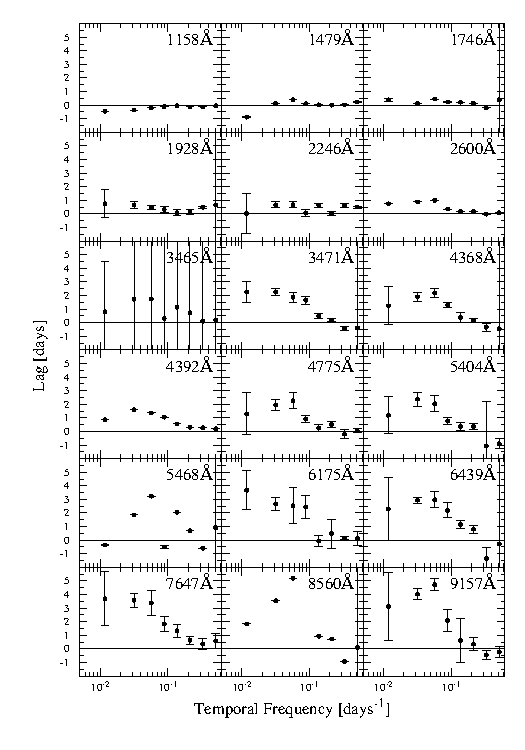
\includegraphics{../img/timelag_atlas_err0.pdf}
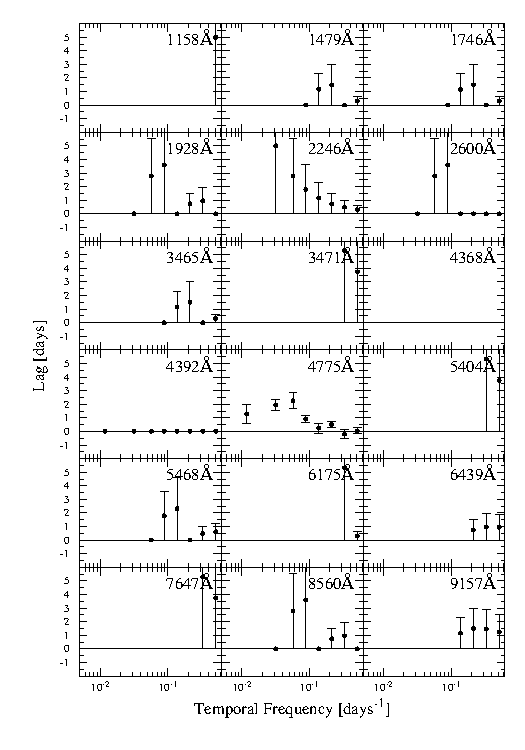
\includegraphics{../img/timelag_atlas_err1.pdf}
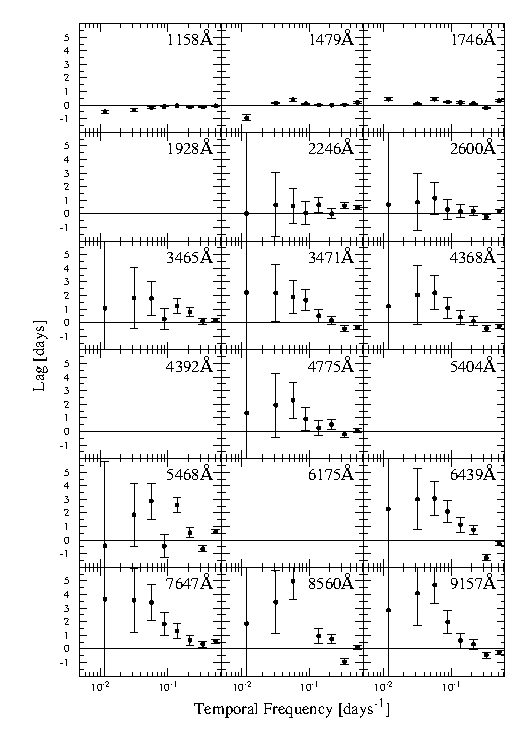
\includegraphics{../img/timelag_atlas_err2.pdf}

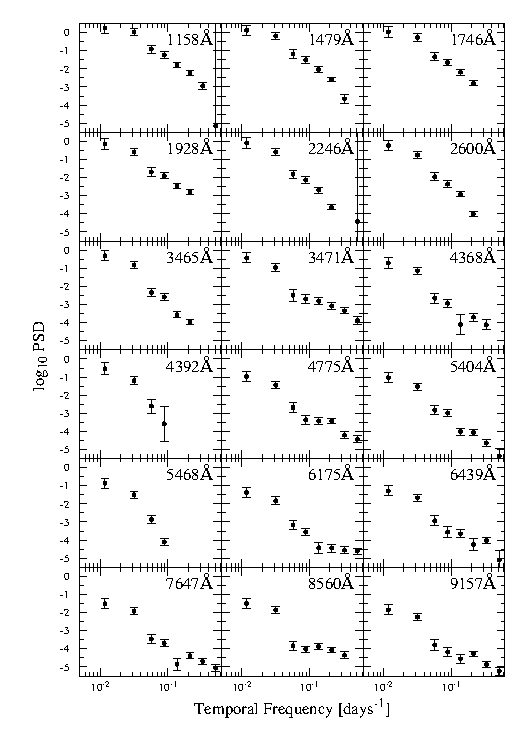
\includegraphics{../img/psd_atlas_err0.pdf}
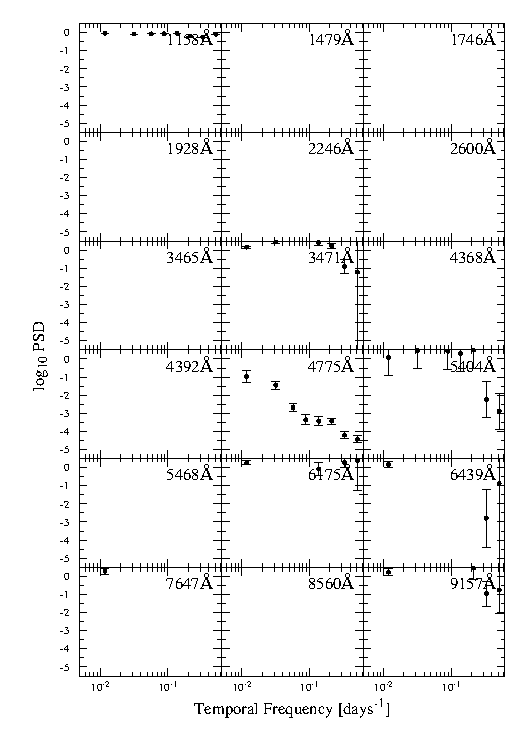
\includegraphics{../img/psd_atlas_err1.pdf}
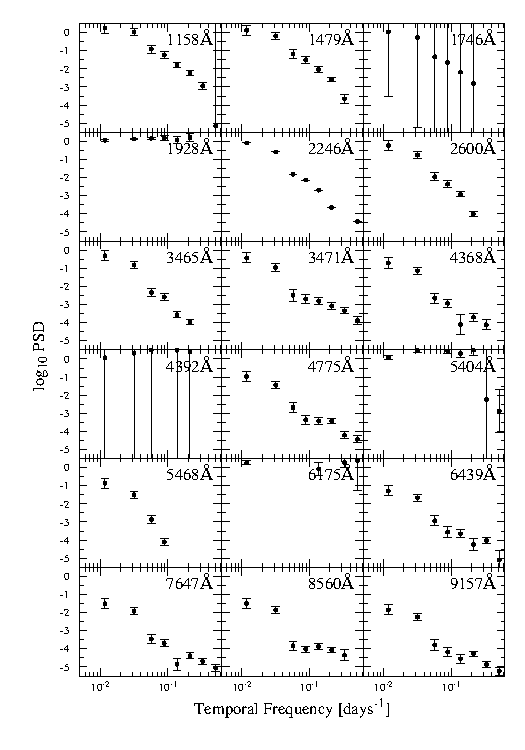
\includegraphics{../img/psd_atlas_err2.pdf}

\end{document}
